Уравнения с частными производными 2-го порядка параболического типа часто встречаются при изучении процессов теплопроводности и диффузии.

\begin{figure}[h!]
    \centering
    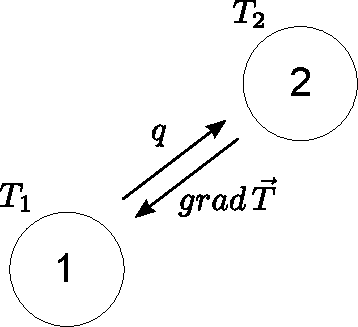
\includegraphics[scale=0.7]{figWarm.pdf}
	
	\label{fig:figWarm}
    \end{figure}
	При постоянных температурах $T_1$ и $T_2$ тепло перетекает от более нагретого участка к менее нагретому. Градиент направлен в сторону возрастания тепла.

\textbf{Закон Фурье}:
\[
	q = - k\, \mathrm{grad} T 
\]
Поток тепла пропорционален градиенту температуры.  $q$ - количество тепла, протекающего за единицу времени через единицу площади.  $q$ --- коэффициент теплопроводности материала.

\begin{wrapfigure}{r}{0.4\textwidth}
	\centering
	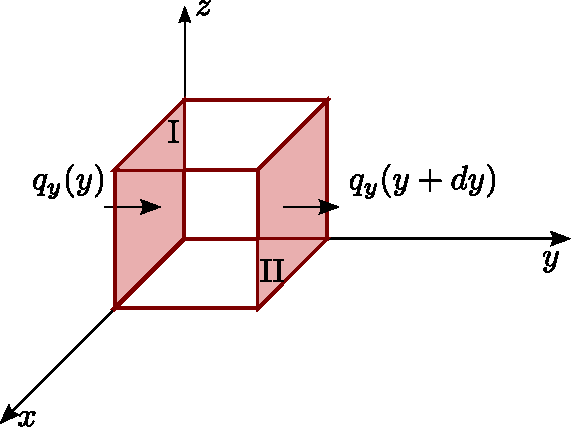
\includegraphics[width=0.4\textwidth]{figWarm2.pdf}
\end{wrapfigure}
Возьмём бесконечно малый объём. Рассмотрим грани куба. Перпендикулярно оси $x$ через грань II выохдит тепловой поток.  Найдём разность между тепловым потоком, вошедшим в I и вышедшим из II.

За время $dt$ в куб входит количество тепла $q_y\, dx dz dt$, а выходит $- q_y(y + dy)\, dx dz dt$.
\[
	q_y(y)\, dx dz dt = - q_y(y + dy)\, dx dz dt 
\]
Мы можем разложить функцию в ряд Тейлора, пользуясь малостью $dy$:
\[
	q_y(y)\, dx dz dt  - q_y(y + dy)\, dx dz dt  - \derp{q_y}{y}{} (y)\, dx dy dz
\]
Пренебрегая малыми 2-го порядка мы получили формулу тепла, которое осталось внутри куба.
\[
	\left(-\derp{}{x}{} q_x - \derp{}{y}{} q_y - \derp{}{z}{} q_z \right)\, dx dy dz  dt
\]
Количество тепла, которое нужно сообщить одному телу, чтобы повысить его температуру на $\Delta T$ равно
\[
	Q = c m \Delta T
\]
где $m= c \rho \,dx dy dz dT$.

Подставляем $Q$
\[
	c \rho \, dT dx dy dz = \left(-\derp{}{x}{} q_x - \derp{}{y}{} q_y - \derp{}{z}{} q_z \right)\, dx dy dz  dt.
\]
Приходим к следующей формуле
\[
	c \rho \derp{T}{t}{} = - \left(\derp{}{x}{}q_x + \derp{}{y}{} q_y + \derp{}{z}{} q_z \right)
\]

Из закона Фурье определим проекции $q_x, q_y, q_z$
\[
	\overrightarrow{\mathrm{grad}} T = \derp{T}{x}{} \vec i + \derp{T}{y}{} \vec j + \derp{T}{z}{} \vec k
\]
\[
	q = - k \overrightarrow{\mathrm{grad}} T
\]
\begin{align*}
	&q_x = - k_x \derp{T}{x}{} &q_y = - k_y \derp{T}{y}{} &q_z = - k_z \derp{T}{z}{}
\end{align*}


Наше тело изотропно, то есть зависит от времени
\[
	c \rho \derp{T}{t}{} = \derp{}{x}{} \left(k_x \derp{T}{x}{} \right) + \derp{}{y}{} \left(k_y \right) + \derp{}{z}{} \left(k_z \derp{T}{z}{} \right)
\]
\[
	\derp{T}{t}{} = \frac{k}{c \rho} \left( \derp{T}{x}{2} + \derp{T}{y}{2} + \derp{T}{z}{2} \right), \quad k_x = k_y = k_z = k = const
\]
\[
	\frac{k}{c \rho} = a^2
\]
где $a$ --- коэффициент температуропроводности, а $c$ --- коэффициент теплоёмкости.
Будем рассматривать уравнение в одномерном случае:
\begin{equation}
	\derp{T}{t}{} = a^2\derp{u}{x}{2}
	\label{equ:equWarm2}
\end{equation}
	Уравнение \eqref{equ:equWarm2} называется \textit{уравнением теплопроводности}.
